\documentclass[a4paper,12pt]{report}

\usepackage{cmap}
\usepackage[T2A]{fontenc}
\usepackage[utf8]{inputenc}
\usepackage[english,russian]{babel}
\usepackage{listings}
\usepackage{amsmath}
\usepackage{amsfonts}
\usepackage{float}
\usepackage{csquotes}
\usepackage{hyphenat}

% \usepackage{titlesec}
% \newcommand{\sectionbreak}{\clearpage}

\usepackage{graphicx}
\graphicspath{ {./images/} }

\usepackage{xcolor}
% \usepackage{courier}

\usepackage[
    backend=biber,
    style=alphabetic,
    sorting=ynt
]{biblatex}
\addbibresource{resources.bib}

\definecolor{buzzlightyear}{HTML}{8757A5}
\definecolor{grass}{HTML}{738D06}
\definecolor{sand}{HTML}{F18A2B}
\definecolor{comment}{HTML}{8E908B}

\lstdefinestyle{habrstyle}{
    backgroundcolor=\color{white},   
    commentstyle=\color{comment},
    keywordstyle=\bfseries\color{buzzlightyear},
    numberstyle=\tiny\color{comment},
    stringstyle=\color{grass},
    basicstyle=\ttfamily\footnotesize,
    breakatwhitespace=false,         
    breaklines=true,                 
    captionpos=b,                    
    keepspaces=true,                 
    numbers=left,                    
    numbersep=5pt,                  
    showspaces=false,                
    showstringspaces=false,
    showtabs=false,                  
    tabsize=4
}

\lstset{style=habrstyle}

\author{Луняк Николай}
\title{Лабораторная работа 6}
\date{\today}

\begin{document}
    \maketitle
    \tableofcontents
    \listoffigures
    \lstlistoflistings
    
    \chapter{Асимптотика}
    
    Нужно оценить асимптотику \sloppy{\texttt{analyze1}}, \sloppy{\texttt{analyze2}} и \sloppy{\texttt{fftpack.dct}}. Чтобы это сделать, подадим на вход \sloppy{\texttt{scipy.stats.linregress}} логарифмированные значения размера текущей выборки и затраченного времени (потому что, например, $x \rightarrow x^k \Rightarrow \log(x) \rightarrow k\cdot \log(x)$).
    
    Сначала импортируем накопленные человечеством знания:
    
\begin{lstlisting}[language=Python,caption=Импорты]
from thinkdsp import Signal, Sinusoid, SquareSignal, TriangleSignal, SawtoothSignal, ParabolicSignal
from thinkdsp import normalize, unbias, PI2, decorate
from thinkdsp import Chirp
from thinkdsp import read_wave
from thinkdsp import Spectrum, Wave, UncorrelatedGaussianNoise

import numpy as np
import pandas as pd

from matplotlib import pyplot

import thinkstats2

from scipy.stats import linregress

import scipy
import scipy.fftpack

def analyze1(ys, fs, ts):
    """Analyze a mixture of cosines and return amplitudes.

    Works for the general case where M is not orthogonal.

    ys: wave array
    fs: frequencies in Hz
    ts: times where the signal was evaluated    

    returns: vector of amplitudes
    """
    args = np.outer(ts, fs)
    M = np.cos(PI2 * args)
    amps = np.linalg.solve(M, ys)
    return amps

def analyze2(ys, fs, ts):
    """Analyze a mixture of cosines and return amplitudes.

    Assumes that fs and ts are chosen so that M is orthogonal.

    ys: wave array
    fs: frequencies in Hz
    ts: times where the signal was evaluated    

    returns: vector of amplitudes
    """
    args = np.outer(ts, fs)
    M = np.cos(PI2 * args)
    amps = np.dot(M, ys) / 2
    return amps

def scipy_dct(ys, freqs, ts):
    return scipy.fftpack.dct(ys, type=3)

loglog = dict(xscale='log', yscale='log')

PI2 = np.pi * 2
\end{lstlisting}

    А теперь создадим список проверяемых размеров входных данных, посчитаем время и отобразим все вместе на одном графике.
    
\begin{lstlisting}[language=Python,caption=Замеры]
def run_speed_test(counts, code, noise):
    results = []
    
    for count in counts:
        print(f'For {count} samples:')
        ts = (0.5 + np.arange(count)) / count
        freqs = (0.5 + np.arange(count)) / 2
        ys = noise.ys[:count]
        result = %timeit -r1 -o code(ys, freqs, ts)
        results.append(result)
        
    return [result.best for result in results]

def fit_slope(counts, results):
    x = np.log(counts)
    y = np.log(results)
    return linregress(x, y).slope

signal = UncorrelatedGaussianNoise()
noise = signal.make_wave(duration=1.0, framerate=16384)

print('Testing analyze1...')
counts = 2 ** np.arange(6, 13)
results1 = run_speed_test(counts, analyze1, noise)
slope1 = fit_slope(counts, results1)
print('')

print('Testing analyze2...')
results2 = run_speed_test(counts, analyze2, noise)
slope2 = fit_slope(counts, results2)
print('')

print('Testing scipy_dct...')
results3 = run_speed_test(counts, scipy_dct, noise)
slope3 = fit_slope(counts, results3)

pyplot.plot(counts, results1, label=f'analyze1 (slope: {slope1})')
pyplot.plot(counts, results2, label=f'analyze2 (slope: {slope2})')
pyplot.plot(counts, results3, label=f'fftpack.dct (slope: {slope3})')
decorate(xlabel='Wave length (N)', ylabel='Time (s)', **loglog)
\end{lstlisting}

%     В логе видим:

% \begin{verbatim}
% Testing analyze1...
% For 64 samples:
% 2 ms ± 0 ns per loop (mean ± std. dev. of 1 run, 100 loops each)
% For 128 samples:
% 4.41 ms ± 0 ns per loop (mean ± std. dev. of 1 run, 100 loops each)
% For 256 samples:
% 13.7 ms ± 0 ns per loop (mean ± std. dev. of 1 run, 100 loops each)
% For 512 samples:
% 18.5 ms ± 0 ns per loop (mean ± std. dev. of 1 run, 10 loops each)
% For 1024 samples:
% 62.2 ms ± 0 ns per loop (mean ± std. dev. of 1 run, 10 loops each)
% For 2048 samples:
% 253 ms ± 0 ns per loop (mean ± std. dev. of 1 run, 1 loop each)
% For 4096 samples:
% 1.64 s ± 0 ns per loop (mean ± std. dev. of 1 run, 1 loop each)

% Testing analyze2...
% For 64 samples:
% 74.3 µs ± 0 ns per loop (mean ± std. dev. of 1 run, 10000 loops each)
% For 128 samples:
% 479 µs ± 0 ns per loop (mean ± std. dev. of 1 run, 1000 loops each)
% For 256 samples:
% 1.97 ms ± 0 ns per loop (mean ± std. dev. of 1 run, 1000 loops each)
% For 512 samples:
% 5.46 ms ± 0 ns per loop (mean ± std. dev. of 1 run, 100 loops each)
% For 1024 samples:
% 19.6 ms ± 0 ns per loop (mean ± std. dev. of 1 run, 100 loops each)
% For 2048 samples:
% 74.1 ms ± 0 ns per loop (mean ± std. dev. of 1 run, 10 loops each)
% For 4096 samples:
% 287 ms ± 0 ns per loop (mean ± std. dev. of 1 run, 1 loop each)

% Testing scipy_dct...
% For 64 samples:
% 9.48 µs ± 0 ns per loop (mean ± std. dev. of 1 run, 100000 loops each)
% For 128 samples:
% 9.93 µs ± 0 ns per loop (mean ± std. dev. of 1 run, 100000 loops each)
% For 256 samples:
% 10.8 µs ± 0 ns per loop (mean ± std. dev. of 1 run, 100000 loops each)
% For 512 samples:
% 12.9 µs ± 0 ns per loop (mean ± std. dev. of 1 run, 100000 loops each)
% For 1024 samples:
% 16.5 µs ± 0 ns per loop (mean ± std. dev. of 1 run, 100000 loops each)
% For 2048 samples:
% 25.8 µs ± 0 ns per loop (mean ± std. dev. of 1 run, 10000 loops each)
% For 4096 samples:
% 53.7 µs ± 0 ns per loop (mean ± std. dev. of 1 run, 10000 loops each)
% \end{verbatim}

\begin{lstlisting}[caption=Лог,literate={µ}{$\mu$}1{±}{$\pm$}2]
Testing analyze1...
For 64 samples:
2 ms ± 0 ns per loop (mean ± std. dev. of 1 run, 100 loops each)
For 128 samples:
4.41 ms ± 0 ns per loop (mean ± std. dev. of 1 run, 100 loops each)
For 256 samples:
13.7 ms ± 0 ns per loop (mean ± std. dev. of 1 run, 100 loops each)
For 512 samples:
18.5 ms ± 0 ns per loop (mean ± std. dev. of 1 run, 10 loops each)
For 1024 samples:
62.2 ms ± 0 ns per loop (mean ± std. dev. of 1 run, 10 loops each)
For 2048 samples:
253 ms ± 0 ns per loop (mean ± std. dev. of 1 run, 1 loop each)
For 4096 samples:
1.64 s ± 0 ns per loop (mean ± std. dev. of 1 run, 1 loop each)

Testing analyze2...
For 64 samples:
74.3 µs ± 0 ns per loop (mean ± std. dev. of 1 run, 10000 loops each)
For 128 samples:
479 µs ± 0 ns per loop (mean ± std. dev. of 1 run, 1000 loops each)
For 256 samples:
1.97 ms ± 0 ns per loop (mean ± std. dev. of 1 run, 1000 loops each)
For 512 samples:
5.46 ms ± 0 ns per loop (mean ± std. dev. of 1 run, 100 loops each)
For 1024 samples:
19.6 ms ± 0 ns per loop (mean ± std. dev. of 1 run, 100 loops each)
For 2048 samples:
74.1 ms ± 0 ns per loop (mean ± std. dev. of 1 run, 10 loops each)
For 4096 samples:
287 ms ± 0 ns per loop (mean ± std. dev. of 1 run, 1 loop each)

Testing scipy_dct...
For 64 samples:
9.48 µs ± 0 ns per loop (mean ± std. dev. of 1 run, 100000 loops each)
For 128 samples:
9.93 µs ± 0 ns per loop (mean ± std. dev. of 1 run, 100000 loops each)
For 256 samples:
10.8 µs ± 0 ns per loop (mean ± std. dev. of 1 run, 100000 loops each)
For 512 samples:
12.9 µs ± 0 ns per loop (mean ± std. dev. of 1 run, 100000 loops each)
For 1024 samples:
16.5 µs ± 0 ns per loop (mean ± std. dev. of 1 run, 100000 loops each)
For 2048 samples:
25.8 µs ± 0 ns per loop (mean ± std. dev. of 1 run, 10000 loops each)
For 4096 samples:
53.7 µs ± 0 ns per loop (mean ± std. dev. of 1 run, 10000 loops each)
\end{lstlisting}

    \begin{figure}[H]
        \centering
        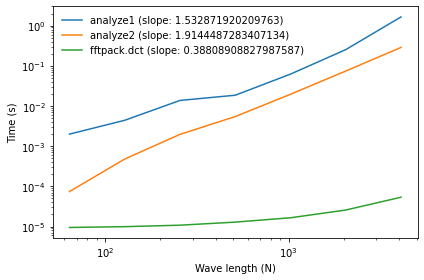
\includegraphics[width=0.75\textwidth]{images/ex1_all.png}
        \caption{Сравнение}
        \label{fig:ex1_all}
    \end{figure}
    
    Похоже, что \sloppy{\texttt{analyze1}} не получилось оценить (возможно, из-за малых размеров выборки), а \sloppy{\texttt{analyze2}} дает ожидаемое значение наклона. 
    
    Последняя функция, \sloppy{\texttt{ffpack.dct}}, оказывается заметно более быстрой по времени, потому что ее сложность пропорциональна $n\log(n)$. \sloppy{\texttt{analyze1}}
    
    \chapter{Сжатие}
    
    Сначаал реализуем простое сжатие для одного небольшого сегмента некоторого звука.
    
\begin{lstlisting}[language=Python,caption=Сжатие сегмента]
def compress(dct, threshold=1, log=False):
    count = 0
    
    for i, amp in enumerate(dct.amps):
        if np.abs(amp) < threshold:
            dct.hs[i] = 0
            count += 1
            
    total = len(dct.amps)
    
    if log:
        print(f'Total: {total}, Removed: {count} = {100 * count / total:.1f}%', sep='\t')
    
    return 100 * count / total
\end{lstlisting}

    Тут просто происходит зануление компонент со \textquote{слишком} малыми амплитудами.
    
    Проверим его на некотором звуке.

\begin{lstlisting}[language=Python,caption=Сжатие сегмента]
wave = read_wave('Sounds/100475__iluppai__saxophone-weep.wav')
segment = wave.segment(start=1.2, duration=0.5)
segment.normalize()

seg_dct = segment.make_dct()
seg_dct.plot(high=4000)
decorate(xlabel='Frequency (Hz)', ylabel='DCT')

pyplot.show()
seg_dct = segment.make_dct()
compress(seg_dct, threshold=100, log=True)
seg_dct.plot(high=4000)
\end{lstlisting}

    \begin{figure}[H]
        \centering
        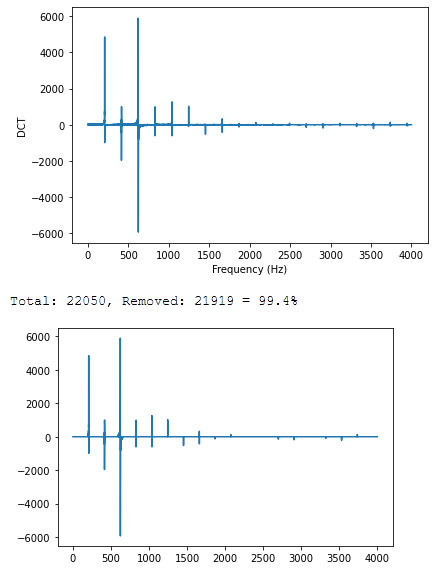
\includegraphics[width=0.75\textwidth]{images/ex2_segment.png}
        \caption{Спектр \textquote{до} и \textquote{после}}
        \label{fig:ex2_segment}
    \end{figure}
    
    Чтобы сжать длинный изменяющийся во времени звук, нам необходимо брать его спектры в течение некоторых сегментов по аналогии с тем, как это делается для спектрограмм. Отсюда следует, что удобно реализовать себе DCT-спектрограмму.
    
\begin{lstlisting}[language=Python,caption=Сжатие длинного звука]
def make_dct_spectrogram(wave, segment_length):
    window = np.hamming(segment_length)
    i, j = 0, segment_length
    step = segment_length // 2
    spectrums = {}

    while j < len(wave.ys):
        segment = wave.slice(i, j)
        segment.window(window)

        t = (segment.start + segment.end) / 2
        spectrums[t] = segment.make_dct()

        i += step
        j += step

    return Spectrogram(spectrums, segment_length)

def compress_by_parts(wave, segment_length):
    spectrogram = make_dct_spectrogram(wave, segment_length=segment_length)
    average = 0
    
    for t, dct in sorted(spectrogram.spec_map.items()):
        average += compress(dct, threshold=0.2)
        
    average /= len(spectrogram.spec_map)
    
    print(f'Average: {average:.1f}%', sep='\t')
    
    return spectrogram

wave2 = compress_by_parts(wave, 512).make_wave()
wave2.make_audio()
\end{lstlisting}

    После запуска лог дает \sloppy{\texttt{Average: 80.9\%}}. На слух звучит примерно так же.
    
    \chapter{Влияние фазы}
    
    Теперь нам нужно запустить готовый \sloppy{\texttt{phase.ipynb}} и посмотреть, что там происходит.
    
    Так как вставлять подробные картинки из notebook'а сюда долго, я лишь опишу процесс словами.
    
    Если мы посмотрим на фазовые сдвиги каждой компоненты некоторого звука, то мы будем видеть только \textquote{нагромождение} случайных значений, однако если отфильтровать частоты с \textquote{незначительными} амплитудами, то начнет вырисовываться струкутра. Величина фазы от частоты компоненты может зависеть как линейно, так и случайно, однако в подавляющем большинстве случаев ухо не будет способно это воспринять. Отсутствие зависимости и \textquote{рандомизацию} уловить еще можно кое-как, но не сдвиг всех компонент по фазе (что в принципе логично, нам не важно, \textquote{когда} мы начали слушать звук). 
    
    Для звуков с \textquote{пропавшей} частотой наблюдается особенность: фазовую структуру таких звуков ухо может воспринимать, однако автор предположил, что это связано с тем, что мозг \textquote{пытается} учесть автокорреляцию.
    
    % \printbibliography
    
\end{document}
